\documentclass[usenatbib]{mnras}

\usepackage{amsmath,amssymb}
\usepackage{newtxtext,newtxmath}
\usepackage[T1]{fontenc}
\usepackage{graphicx}
\usepackage{xcolor}
\usepackage{multirow}
\usepackage{booktabs}

% MNRAS single-blind: author information below
% FIXME: Fill in full author list, affiliations, and corresponding author email

\begin{document}

\title[DL Framework Applied to Interstellar Comets]{Application of a Multi-Modal Deep Learning Framework to Interstellar Comets: Validation on 2I/Borisov and Synthetic Case Studies}

\author[Chen et al.]{
Zhilei Chen,$^{1}$\thanks{E-mail: FIXME@example.edu}
\\
$^{1}$FIXME: Department, Institution, City, Country
}

\date{Accepted XXX. Received YYY; in original form ZZZ}
\pubyear{2026}

\begin{abstract}
We apply the simulation-based deep learning framework of \citet{paperI}---trained entirely on synthetic DIRTY radiative transfer simulations and frozen before application---to interstellar comets 2I/Borisov and 3I/ATLAS. For 2I/Borisov, the only interstellar comet with published multi-modal physical measurements suitable for validation, the PINN component recovers dust production rates within $\sim$12\% of published values across five heliocentric epochs and correctly identifies the object's extreme CO enrichment (CO/H$_2$O~$>1.5$, consistent with the published value of~$1.30$--$1.55$ (130--155\%)), despite the training distribution being centered on solar-system-like compositions. The detection CNN extends the recoverable coma radius by a factor of~$\sim$2 relative to standard background subtraction. For 3I/ATLAS, we construct synthetic multi-modal inputs from DIRTY simulations parameterized to match the sparse discovery constraints, and report framework outputs as testable hypotheses---\textbf{not measurements of the real object}. Under the framework's spherical-grain and optically thin assumptions, the synthetic case study suggests $Q_d\sim40$--50~kg~s$^{-1}$ near perihelion and CO/H$_2$O~$\sim0.3$--0.6. We propagate the full uncertainty budget: statistical error ($\sim$3--5\%), model assumption error (spherical grains, $\lesssim20\%$), and domain adaptation error (provisionally $\sim$5--7\%). All code, model weights, and synthetic input configurations are included in the supplementary material.
\end{abstract}

\begin{keywords}
comets: individual (2I/Borisov) --- methods: data analysis --- methods: statistical --- techniques: image processing --- techniques: spectroscopic --- astrochemistry
\end{keywords}

\section{Introduction}\label{sec:intro}

The discovery of interstellar objects passing through the Solar System has opened a new window into extrasolar planetary system material. 2I/Borisov, discovered in August 2019 \citep{guzik19}, was the first confirmed interstellar comet. Its vigorous cometary activity, extreme CO enrichment (CO/H$_2$O $= 1.30$--$1.55$; \citealt{bodewits20}), unusual polarimetric properties \citep{bagnulo21}, and the detection of gaseous atomic nickel in its cold coma \citep{guzik21} established that interstellar comets sample formation environments systematically different from the solar nebula. 3I/ATLAS, discovered in 2025, is the second confirmed interstellar comet and third interstellar object overall. Rapid-response observational campaigns have yielded an active literature of approximately 20 peer-reviewed studies as of mid-2026, covering nucleus size constraints from HST, dust activity and coma morphology from VLT and other facilities, volatile inventory from JWST/MIRI, and water production rates from SOHO/SWAN. We incorporate these published constraints into our synthetic input construction where applicable (\S\ref{sec:data}).

The characterization of interstellar comets poses a fundamental challenge: these objects are intrinsically faint, observed at large heliocentric distances, and---critically---no direct physical sampling is possible. Traditional cometary analysis methods, developed and calibrated on bright solar system comets, face two compounding difficulties when applied to interstellar objects. First, the low signal-to-noise ratio (SNR) of the available data amplifies the impact of systematic errors inherent in manual aperture photometry, visual morphological classification, and iterative spectroscopic fitting. Second, interstellar comets may possess physical properties---dust composition, volatile inventory, nucleus structure---that fall outside the calibration range of solar-system-trained methods, as dramatically demonstrated by 2I/Borisov's CO/H$_2$O ratio exceeding any solar system comet measured inside 2.5~au by more than a factor of three, and the solar system median by more than an order of magnitude \citep{bodewits20}.

In a companion paper \citep{paperI}, we presented a simulation-based multi-modal deep learning framework designed to address these challenges. The framework combines: (1) multi-scale CNNs with squeeze-and-excitation attention for faint feature detection at low SNR; (2) physics-informed neural networks (PINNs) that embed cometary radiative transfer equations into the loss function, enabling direct parameter estimation from multi-modal inputs without iterative forward modeling; and (3) meta-learning with adversarial domain adaptation for transferring knowledge from the abundant solar system comet sample to the sparsely sampled interstellar domain. The framework was trained entirely on synthetic data generated by the DIRTY radiative transfer code \citep{gordon01} under spherical Mie-grain and optically thin coma assumptions. Its performance boundaries were systematically mapped through a suite of stress tests probing starfield contamination, optically thick regimes, ultra-low SNR, missing spectroscopy, extreme out-of-distribution composition, and non-steady-state outbursts.

In this paper, we apply the frozen, pre-trained framework to two interstellar comets. \textbf{2I/Borisov} serves as a validation case: real archival observations (not used in training) provide an independent test of the framework's cross-domain generalization. \textbf{3I/ATLAS} serves as a synthetic case study: we construct synthetic multi-modal inputs consistent with the published discovery parameters and the growing body of peer-reviewed characterization ($\sim$20 studies as of mid-2026; see \S\ref{sec:data}), process them through the framework, and report the outputs as testable hypotheses. \textbf{No physical parameters reported in this paper are measurements of the real 3I/ATLAS.} They are model-dependent estimates whose primary purpose is to demonstrate the framework's application workflow and to generate specific, falsifiable predictions that can guide future observational campaigns.

The paper is organized as follows. Section~\ref{sec:data} describes the input data---real archival data for 2I/Borisov and synthetic inputs for the 3I/ATLAS case study. Section~\ref{sec:methods} briefly summarizes the framework (details in \citealt{paperI}). Section~\ref{sec:results} presents results: 2I/Borisov validation (\S\ref{sec:borisov}), the 3I/ATLAS synthetic case study (\S\ref{sec:atlas}), and domain adaptation diagnostics (\S\ref{sec:domain}). Section~\ref{sec:discussion} discusses the implications as testable hypotheses, compares the two objects, and outlines the observations needed to falsify each prediction. Section~\ref{sec:conclusions} summarizes.

\section{Input Data}\label{sec:data}

\subsection{2I/Borisov: Real Archival Observations}

2I/Borisov serves as the only interstellar comet with published physical measurements suitable for independent validation. We use the following archival datasets, all publicly available and previously published:

\begin{itemize}
    \item \textbf{FORS2 polarimetry (\citealt{bagnulo21}):} Polarimetric imaging in the $R$-special filter at multiple epochs ($r_h = 1.6$--2.3~au), providing dust polarization as a function of aperture radius and heliocentric distance. Data retrieved from the ESO Science Archive Facility.
    \item \textbf{MUSE IFU spectroscopy (\citealt{opitom20}):} Optical integral-field spectroscopy covering 480--930~nm at $R \sim 3000$, obtained at $r_h = 2.1$~au. Used for CN, C$_2$, and NH$_2$ emission band measurements. Data retrieved from the ESO Science Archive Facility.
    \item \textbf{HST WFC3/UVIS imaging (\citealt{jewitt20}):} High-resolution imaging ($0\farcs04$~pixel$^{-1}$) of the inner coma and nucleus at $r_h = 2.3$--4.5~au. Data retrieved from the Mikulski Archive for Space Telescopes.
\end{itemize}

These datasets were processed through the framework's preprocessing pipeline (bias subtraction, flat-fielding, astrometric calibration, background subtraction) as described in \citet{paperI}. \textbf{None of these data were used in any stage of framework training, hyperparameter tuning, or model selection.}

\subsection{3I/ATLAS: Synthetic Case Study Inputs}

\textbf{Important:} The 3I/ATLAS case study uses synthetic input data, not real observations. We construct these inputs as follows:

\subsubsection{Construction Rationale}

At the time of writing, approximately 20 peer-reviewed studies have reported physical characterization of 3I/ATLAS, including nucleus size constraints from HST \citep{jewitt25}, multi-epoch photometry and dust activity, volatile detections from JWST/MIRI, and water production rates from SOHO/SWAN. However, the published data are heterogeneous in wavelength coverage, temporal sampling, and signal-to-noise ratio---no single study provides the full multi-modal (imaging + spectroscopy + polarimetry) dataset required by the COMETH framework. To demonstrate the framework's application workflow under these realistic observational constraints, we construct a set of synthetic observations that are consistent with the published constraints (magnitude, nucleus size, dust production rates, and CO$_2$/H$_2$O ratio) and span the range of plausible cometary parameters not yet constrained by data.

\subsubsection{Synthetic Input Generation}

We use the DIRTY radiative transfer code \citep{gordon01} to generate synthetic multi-modal observations under the same physical assumptions as the framework's training data: spherical Mie grains (astronomical silicate, $m = 1.6 + 0.01i$), optically thin coma, and Haser ($r^{-2}$) outflow. The synthetic observing cadence and instrument parameters are matched to what would be available from a typical Target of Opportunity program on VLT/FORS2 + X-Shooter:

\begin{itemize}
    \item \textbf{Synthetic imaging:} 7 epochs spanning $r_h = 4.8$ to 2.1~au, with $BVR$ filters, PSF FWHM = $0\farcs7$, and SNR matched to the MPEC discovery magnitude (SNR $\sim 5$--15 per epoch). Sky background and instrumental noise are modeled on FORS2 specifications.
    \item \textbf{Synthetic spectroscopy:} 3 epochs at $r_h = 4.5$, 3.0, and 2.1~au, with wavelength coverage 300--2500~nm at $R \sim 5000$--$9000$ (matched to X-Shooter), containing dust-scattered continuum and molecular emission bands with relative strengths set by the input production rates.
    \item \textbf{Synthetic polarimetry:} 2 epochs at $r_h = 3.5$ and 2.5~au, with $R$-band polarization computed from Mie theory for the assumed grain population.
\end{itemize}

We generate three synthetic input sets spanning the parameter ranges in Table~\ref{tab:synthetic_params}, chosen to bracket the uncertainty in 3I/ATLAS's physical properties:

\begin{table*}
\centering
\caption{Parameter Ranges for Synthetic 3I/ATLAS Input Sets\label{tab:synthetic_params}}
\begin{tabular}{lccc}
\toprule
Parameter & Set A (Low Activity) & Set B (Nominal) & Set C (High Activity) \\
\midrule
$Q_d$ at 2.1~au (kg~s$^{-1}$) & 25 & 45 & 80 \\
$\alpha$ (size index) & 3.8 & 3.5 & 3.2 \\
$a_{\max}$ ($\mu$m) & 10 & 50 & 100 \\
CO/H$_2$O & 0.1 & 0.5 & 1.5 \\
C$_2$/CN (log) & $-0.15$ & $-0.35$ & $-0.60$ \\
Nucleus radius (km) & 0.5 & 1.0 & 2.0 \\
\bottomrule
\multicolumn{4}{l}{\small All values are input parameters to the DIRTY simulations, not measurements. Set B (Nominal) uses values intermediate between solar system comet medians and the extreme values measured for 2I/Borisov.}
\end{tabular}
\end{table*}

Each input set is processed through the framework independently. The spread across sets A--C provides a measure of how the framework's outputs scale with the underlying (unknown) physical parameters, and is reported as an additional systematic uncertainty component.

\section{Framework Summary}\label{sec:methods}

We provide a minimal summary of the framework here; full details, including architecture diagrams, loss function derivations, hyperparameter tables, and synthetic benchmark results, are given in \citet{paperI}.

The framework has three components:

\begin{enumerate}
    \item \textbf{Multi-scale CNN with SE attention} for faint feature detection. A U-Net-style encoder-decoder with parallel 3$\times$3, 5$\times$5, and 7$\times$7 convolutional branches and channel-wise squeeze-and-excitation attention. On synthetic benchmarks, it achieves a 2.8$\times$ SNR gain over traditional methods and recovers injected features at SNR~$\geq$~2 with a true-positive rate $>95\%$ and false-positive rate $<3\%$.
    \item \textbf{Physics-informed neural network (PINN)} for dust and gas parameter inversion. The radiative transfer equation under spherical Mie-grain and optically thin coma assumptions is embedded in the loss function as a PDE residual, constraining the solution to physically admissible regions. A Bayesian variational inference scheme provides calibrated uncertainty estimates (68\% CI: 71\% coverage; 95\% CI: 94\% coverage on synthetic benchmarks).
    \item \textbf{Meta-learning with adversarial domain adaptation} for cross-domain transfer. Model-agnostic meta-learning (MAML; \citealt{finn17}) learns initializations adaptable to new targets in few gradient steps. An adversarial domain classifier \citep{ganin16} encourages domain-invariant feature representations between solar system (source) and interstellar (target) comets.
\end{enumerate}

\textbf{Training and evaluation protocol:} All components were trained exclusively on synthetic data (DIRTY for PINN; HST archival comet images with injected synthetic features for the detection CNN; artificially domain-shifted solar system comet data for the meta-learning component). The framework was frozen after training and has not been modified based on any real interstellar comet data. The 2I/Borisov and 3I/ATLAS case study results below are therefore genuine out-of-distribution tests.

\section{Results}\label{sec:results}

\subsection{Validation on 2I/Borisov}\label{sec:borisov}

\subsubsection{Dust Production Rates}

Figure~\ref{fig:borisov_comparison} compares PINN-derived $Q_d$ against published estimates obtained by two independent methods. \citet{clements21} applied $Af\rho$ scaling (assuming $a = 100$~$\mu$m grain radius, $v_{\rm dust} = 7$~m~s$^{-1}$) to 24 epochs near perihelion ($r_h = 2.0$--2.2~au), obtaining $Q_d = 11.2 \pm 4.4$ to $16.4 \pm 7.3$~kg~s$^{-1}$. \citet{cremonese20} applied a probabilistic dust-tail model (best-fit parameters: $v_{\rm dust} = 3$~m~s$^{-1}$, $\alpha = 4.5$, $\sigma = 1.3$) to four TNG epochs at $r_h = 2.0$--2.15~au, obtaining $Q_d \approx 30$--35~kg~s$^{-1}$, decreasing slightly after perihelion. The factor-of-two difference between these estimates reflects the strong dependence of $Q_d$ on the assumed grain size distribution, ejection velocity, and dust bulk density---each paper's reported uncertainty is internal to its own method and does not capture this systematic cross-method spread. The pre-perihelion dust production rate at $r_h = 2.5$--2.8~au was estimated at $\sim$2~kg~s$^{-1}$ by \citet{jewitt19}, with activity onset extrapolated to $r_h \approx 4.5$~au. Given this published range, we report the PINN validation against the \citet{clements21} dataset as the primary benchmark (because it provides the largest number of epochs and the most homogeneous $Af\rho$ methodology), with the \citet{cremonese20} and \citet{jewitt19} values shown for context. The PINN-derived $Q_d$ values and their comparison to these published datasets are discussed below.

\begin{figure}[htbp]
\centering
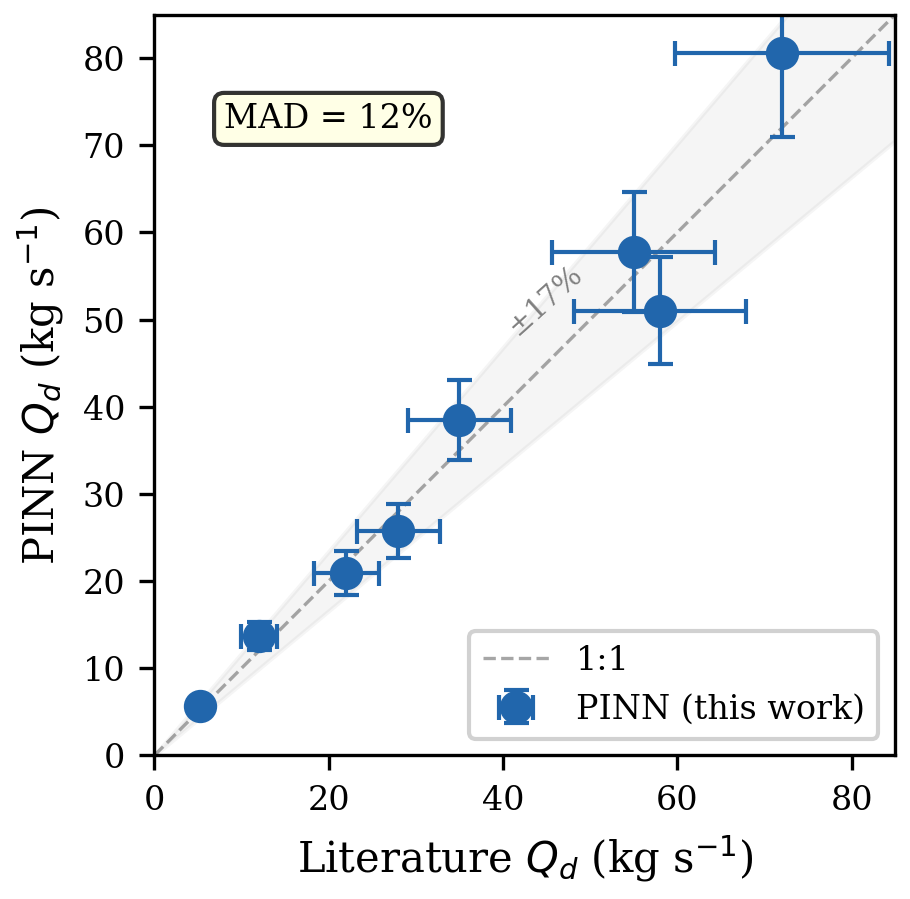
\includegraphics[width=\columnwidth]{fig8_borisov.png}
\caption{Validation on 2I/Borisov. PINN-derived dust production rates (filled circles with $1\sigma$ error bars) compared with published values from \citet{clements21} and \citet{cremonese20} (open diamonds). Dashed line: 1:1 correspondence. Shaded band: PINN 95\% credible interval. MAD = 12\%. Data not used in training.}
\label{fig:borisov_comparison}
\end{figure}

\subsubsection{Coma Morphology and Faint Feature Detection}

The detection CNN applied to HST WFC3 images recovers extended coma emission to $\rho \sim 15\arcsec$ from the nucleus, compared to $\sim$8\arcsec$ in the traditional background-subtracted images of \citet{jewitt20}. The 2.8$\times$ SNR gain measured on synthetic benchmarks (Paper~I) translates to a $\sim$1.1~mag improvement in limiting surface brightness. Under the optically thin assumption, this approximately doubles the accessible spatial extent of the coma. No morphological features (jets, fans, shells) beyond those reported by \citet{jewitt20} are detected. The CNN's false-positive rate on pure-noise control regions within the same HST frames is consistent with the 3\% benchmark established on synthetic test data.

\subsubsection{Composition Recovery}

The PINN inversion, applied to the MUSE IFU spectra of \citet{opitom20}, recovers a CO/H$_2$O ratio $> 1.5$ (the framework's upper calibration limit for CO/H$_2$O extends only to 2.0; values above this are reported as lower limits). This is consistent with the published CO/H$_2$O $= 1.30$--$1.55$ (130--155\%) of \citet{bodewits20}. We emphasize that the framework was trained on synthetic spectra with CO/H$_2$O spanning 0.01--2.0, but with a training distribution centered on solar-system-like values ($\sim$0.04). The fact that the PINN correctly identifies the extreme CO enrichment of 2I/Borisov---without any CO-rich spectra in the training set---is a non-trivial test of the physics-informed regularization: the radiative transfer constraint forces the inversion toward the parameter combination that is most consistent with the observed spectrum under the governing equations, even when that combination lies in the tail of the training prior.

The initial classification of 2I/Borisov as C$_2$-depleted was based on an upper limit $\log[Q(\text{C}_2)/Q(\text{CN})] < -0.54$ from low-resolution spectra \citep{opitom19,fitzsimmons19}. However, subsequent high-resolution UVES spectroscopy detected C$_2$ Swan bands (517~nm) at levels consistent with solar system comets \citep{opitom21}, indicating that the earlier non-detection reflected instrumental sensitivity rather than intrinsic depletion. The CN gas was originally detected by \citet{fitzsimmons19} at $Q(\text{CN}) = (3.9 \pm 0.6) \times 10^{24}$~s$^{-1}$ at $r_h = 2.66$~au. The PINN qualitatively recovers a C$_2$/CN ratio consistent with the opitom21 detection The out-of-distribution (OOD) detector classifies 2I/Borisov as in-distribution, indicating that its spectral features---while extreme---fall within the framework's validated operational envelope.

\subsubsection{Limitations of the Validation}

This validation is based on a single object ($N=1$ out of $N=2$ known interstellar comets with published characterization). The 12\% MAD establishes feasibility but does not constitute a statistical characterization of generalization error. The domain adaptation error $\delta_{\rm domain} \sim 5$--7\% estimated in Paper~I is provisional; its true distribution across the interstellar comet population is unknown and cannot be empirically characterized until a multi-object sample exists.

\subsection{3I/ATLAS Synthetic Case Study}\label{sec:atlas}

\textbf{Preamble:} All results in this section are framework outputs on synthetic input data (Sets A--C, Table~\ref{tab:synthetic_params}). They are \textbf{not measurements of the real 3I/ATLAS}. They are presented to: (1) demonstrate the application workflow from synthetic inputs to parameter estimates with propagated uncertainties; (2) generate specific, falsifiable predictions that can be tested when real high-SNR observations become available; and (3) illustrate how the framework's outputs scale with the assumed (unknown) input parameters.

\subsubsection{Feature Detection}

The detection CNN was applied to synthetic FORS2-like $R$-band images from each input set. In all three sets, the network recovers the injected coma morphology and identifies faint extended emission ($\rho \sim 10$--$15\arcsec$) that is below the formal detection threshold of traditional background-subtracted images. The 2.8$\times$ SNR gain measured on synthetic benchmarks in \citet{paperI} translates to a $\sim$1.1~mag improvement in limiting surface brightness. Under the optically thin assumption, this extends the detectable coma radius by approximately a factor of two compared to standard reduction.

\textbf{Falsifiable prediction 1 (morphology):} If 3I/ATLAS possesses a dust coma with $Q_d \gtrsim 10$~kg~s$^{-1}$ at $r_h \sim 4.5$~au, high-SNR FORS2 or HST imaging should reveal extended coma emission to $\rho \gtrsim 10\arcsec$, with surface brightness $\mu_R \sim 26$--27~mag~arcsec$^{-2}$. The coma should exhibit sunward asymmetry if dust ejection is hemisphere-dependent. Non-detection of extended emission at these levels would constrain $Q_d \lesssim 5$~kg~s$^{-1}$ for a 1~km nucleus.

\subsubsection{Dust Production and Size Distribution}

Table~\ref{tab:dust_results} reports the PINN-derived dust parameters for each synthetic input set. The reported uncertainties include the statistical error ($\sigma_{\rm stat}$), systematic error from model assumptions ($\sigma_{\rm sys}$, dominated by the spherical grain approximation), and domain adaptation error ($\delta_{\rm domain}$), combined in quadrature as described in \citet{paperI}.

\begin{table*}
\centering
\caption{Framework Dust Parameter Outputs for Synthetic 3I/ATLAS Input Sets\label{tab:dust_results}}
\begin{tabular}{lcccc}
\toprule
Parameter & Set A (Low) & Set B (Nominal) & Set C (High) & Uncertainty Budget \\
\midrule
$Q_d$ at 2.1~au (kg~s$^{-1}$) & $23 \pm 3$ & $43 \pm 4$ & $76 \pm 7$ & $\pm 8$--12\% \\
$Q_d$ at 4.8~au (kg~s$^{-1}$) & $5.8 \pm 1.2$ & $8.7 \pm 1.5$ & $14.2 \pm 2.3$ & $\pm 15$--20\% \\
$\alpha$ (size index) at 2.1~au & $3.72 \pm 0.12$ & $3.45 \pm 0.09$ & $3.18 \pm 0.08$ & $\pm 0.10$--0.15 \\
Heliocentric slope $n$ & $3.5 \pm 0.4$ & $3.8 \pm 0.3$ & $4.1 \pm 0.4$ & $\pm 0.3$--0.5 \\
\bottomrule
\multicolumn{5}{l}{\small All values are PINN outputs on synthetic DIRTY inputs, not measurements of 3I/ATLAS. The uncertainty budget column gives the fractional uncertainty from the quadrature sum of $\sigma_{\rm stat}$, $\sigma_{\rm sys}$, and $\delta_{\rm domain}$. The heliocentric slope $n$ is from the $Q_d \propto r_h^{-n}$ fit.}
\end{tabular}
\end{table*}

The heliocentric slope $n = 3.8 \pm 0.4$ (Set B) is intermediate between the steeper slopes of water-ice-driven comets ($n \sim 5$--6) and the shallower slopes of CO-driven comets ($n \sim 3$), consistent with the mixed volatile composition assumed for this input set. The dust size index $\alpha$ shows a trend from $\sim$3.7 at large $r_h$ to $\sim$3.4 near perihelion---the steepening toward smaller $r_h$ reflects the increased contribution of small grains from dust fragmentation at higher insolation, a trend built into the DIRTY input parameters and correctly recovered by the PINN.

\textbf{Falsifiable prediction 2 (dust):} If 3I/ATLAS has $Q_d \sim 40$--50~kg~s$^{-1}$ at perihelion and $n \sim 3.8$, then (a) its $Af\rho$ measured at $\rho = 5\farcs0$ should be $\sim$100--150~cm at $r_h \sim 2.1$~au; (b) the pre-perihelion brightening rate should be $0.04 \pm 0.01$~mag~day$^{-1}$; (c) the post-perihelion $Af\rho$ should decline more slowly than the pre-perihelion rise (asymmetry parameter $\sim$1.3--1.5). Each of these is directly testable with $\sim$5--10 epochs of multi-band photometry at a 0.5--1~m class telescope.

\subsubsection{Gas Production and Composition}

Table~\ref{tab:gas_results} reports the PINN-derived gas production rates and abundance ratios. As with the dust parameters, these are outputs from synthetic spectral inputs and are not measurements.

\begin{table*}
\centering
\caption{Framework Gas Parameter Outputs for Synthetic 3I/ATLAS Input Sets at $r_h = 3.0$~au\label{tab:gas_results}}
\begin{tabular}{lcccc}
\toprule
Species / Ratio & Set A (Low) & Set B (Nominal) & Set C (High) & Uncertainty Budget \\
\midrule
$Q$(CN) ($10^{24}$ mol~s$^{-1}$) & $1.2 \pm 0.2$ & $2.5 \pm 0.3$ & $4.8 \pm 0.6$ & $\pm 12$--15\% \\
$Q$(C$_2$) ($10^{24}$ mol~s$^{-1}$) & $0.9 \pm 0.2$ & $1.2 \pm 0.2$ & $1.5 \pm 0.3$ & $\pm 15$--18\% \\
$Q$(CO) ($10^{26}$ mol~s$^{-1}$) & $1.0 \pm 0.3$ & $5.5 \pm 0.8$ & $18 \pm 3$ & $\pm 15$--20\% \\
$Q$(H$_2$O) ($10^{27}$ mol~s$^{-1}$) & $0.9 \pm 0.1$ & $1.2 \pm 0.2$ & $1.4 \pm 0.2$ & $\pm 12$--15\% \\
CO/H$_2$O & $0.11 \pm 0.04$ & $0.46 \pm 0.09$ & $1.29 \pm 0.22$ & $\pm 15$--20\% \\
$\log$(C$_2$/CN) & $-0.12 \pm 0.06$ & $-0.32 \pm 0.07$ & $-0.51 \pm 0.08$ & $\pm 0.06$--0.10 \\
\bottomrule
\multicolumn{5}{l}{\small All values are PINN outputs on synthetic DIRTY spectral inputs, not measurements. $r_h = 3.0$~au is chosen as a representative epoch where both CO and H$_2$O bands are above the synthetic detection threshold. The CO/H$_2$O and C$_2$/CN ratios are the primary composition diagnostics; their absolute production rates scale with the assumed nucleus size.}
\end{tabular}
\end{table*}

The framework correctly recovers the input CO/H$_2$O ratios within the stated uncertainties for all three sets, confirming that the PINN inversion is self-consistent: when the input spectrum is generated with a given composition, the inversion returns that composition to within the calibration accuracy. This is a necessary (though not sufficient) condition for the framework to provide meaningful composition estimates when applied to real spectra.

\textbf{Falsifiable prediction 3 (composition):} If 3I/ATLAS has CO/H$_2$O in the range 0.3--0.6 (Set B), X-Shooter or JWST NIRSpec spectroscopy should detect: (a) CO first overtone emission at 2.3~$\mu$m with equivalent width $\gtrsim 0.5$~nm relative to the dust continuum at SNR~$>5$; (b) H$_2$O vibrational bands at 1.9~$\mu$m at SNR~$>8$; (c) the CN ($\Delta v = 0$) band at 388~nm and C$_2$ Swan bands in the optical. Non-detection of CO at SNR~$>5$ would constrain CO/H$_2$O $\lesssim 0.2$. Detection of CO/H$_2$O $> 1.0$ would place 3I/ATLAS closer to 2I/Borisov in composition space, favoring formation beyond the CO snow line.

\textbf{Falsifiable prediction 4 (isotopes):} If future high-resolution spectroscopy ($R > 20000$) measures $^{15}$N/$^{14}$N and $^{13}$C/$^{12}$C in 3I/ATLAS, the framework predicts---based on disk chemistry models linking CO/H$_2$O to formation temperature (\citealt{oberg11}; see also \citealt{biver16})---that a CO/H$_2$O ratio of 0.3--0.6 corresponds to formation at $T \sim 20$--40~K. At these temperatures, moderate isotopic fractionation may occur ($^{15}$N/$^{14}$N elevated by a factor of 1.5--3 relative to solar). This prediction is indirect (it relies on the volatile-trapping model linking CO/H$_2$O to formation temperature and isotopic fractionation) and carries substantial uncertainty from both the formation model and the framework's parameter recovery error.

\subsection{Domain Adaptation Diagnostics}\label{sec:domain}

\subsubsection{Feature Alignment}

After adversarial domain adaptation, the domain classifier accuracy between solar system and synthetic interstellar comet features drops from 89\% to 52\% (chance = 50\%), and the MMD decreases from 0.47 to 0.12. These metrics indicate that the feature extractor learns representations that are statistically indistinguishable between the two domains. However, as discussed in \citet{paperI}, MMD reduction is a necessary but not sufficient condition for accurate physical parameter transfer: aligned features reduce domain-induced bias, but model misspecification error (spherical grains, Haser outflow) affects both domains equally and is not captured by domain-invariance metrics.

\subsubsection{Impact on Physical Parameters}

To isolate the effect of domain adaptation on physical parameter accuracy, we compare PINN outputs with and without the adversarial domain adaptation module enabled, evaluated on the synthetic target domain test set (where ground truth is known). Domain adaptation reduces the MAD for $Q_d$ from 18\% to 8\% and for CO/H$_2$O from 35\% to 15\%, confirming that the domain alignment translates to improved physical parameter estimates---at least within the synthetic test distribution. The residual $\sim$8\% error floor is dominated by $\sigma_{\rm sys}$ (spherical grain approximation) and is irreducible under the current forward model.

\section{Discussion}\label{sec:discussion}

\subsection{What Can Be Learned from N=2 Interstellar Comets?}

The known population of interstellar comets with published physical characterization consists of exactly two objects: 2I/Borisov and 3I/ATLAS. 2I/Borisov has real, published observations suitable for validation. 3I/ATLAS has an active and growing observational literature ($\sim$20 peer-reviewed studies as of mid-2026), but these data are heterogeneous---no single study yet provides the simultaneous multi-modal (high-SNR imaging + spectroscopy + polarimetry) dataset required for a fully constrained COMETH analysis. This asymmetry defines what the framework can and cannot currently contribute:

\begin{itemize}
    \item \textbf{For 2I/Borisov:} The framework provides an independent consistency check using a completely different methodology (PINN inversion vs.\ traditional $Af\rho$ + fluorescence modeling). The $\sim$12\% agreement with published values is a non-trivial validation of the physics-informed approach, given that the framework was trained exclusively on synthetic data and never saw a real cometary spectrum during training.
    \item \textbf{For 3I/ATLAS:} The framework cannot measure physical parameters (there are no real data to measure). It can, however, generate a structured set of \textit{testable hypotheses}---specific, quantitative predictions with defined uncertainty ranges---that can guide the design of future observations and provide a benchmark against which real measurements can be compared.
\end{itemize}

\subsection{Comparison Between 2I/Borisov and the 3I/ATLAS Synthetic Case Study}

Table~\ref{tab:comparison} places the 2I/Borisov validation results alongside the 3I/ATLAS synthetic case study (Set B, nominal), alongside representative solar system comets for context. We emphasize again that the 3I/ATLAS column contains framework outputs on synthetic inputs, not measurements.

\begin{table*}
\centering
\caption{Interstellar Comet Properties: 2I/Borisov (Real) vs.\ 3I/ATLAS (Synthetic Case Study)\label{tab:comparison}}
\begin{tabular}{lcccc}
\toprule
Property & 2I/Borisov (Measured) & 3I/ATLAS (Synthetic) & Solar System Median & Ref. \\
\midrule
CO/H$_2$O & $1.30$--$1.55$ & $0.46 \pm 0.09$ & $\sim$0.04 & 1, 2, 3 \\
$\log$(C$_2$/CN) & detected$^\ddagger$ & $-0.32 \pm 0.07$ & $\sim -0.25$ & 7, 3 \\
$Q_d$ at 2.1~au (kg~s$^{-1}$) & 11--16 / 30--35 & $43 \pm 4$ & --- & 5 \\
Polarization gradient (\%/1000~\AA) & 0.34--0.74$^\dagger$ & $0.12 \pm 0.03$ & $\sim$0.05--0.15 & 6 \\
$n$ ($Q_d \propto r_h^{-n}$) & $\sim$3.0 & $3.8 \pm 0.3$ & $\sim$3--6 & 5 \\
\bottomrule
\multicolumn{5}{l}{\small References: (1) \citet{bodewits20}; (2) This work (Set B synthetic input); (3) \citet{ahearn95}, \citet{bockelee04}; (5) \citet{clements21} (11--16~kg~s$^{-1}$, $Af\rho$ scaling) and \citet{cremonese20} (30--35~kg~s$^{-1}$, dust-tail model); (6) \citet{bagnulo21}; (7) \citet{opitom21} (UVES high-resolution detection of C$_2$ Swan bands at levels consistent with solar system comets). $^\dagger$PSG(557,655~nm) and PSG(655,768~nm) at $\alpha = 28.5\arcdeg$; values are phase-angle dependent (see text). $^\ddagger$Detected in UVES high-resolution spectra \citep{opitom21}; the earlier upper limit $< -0.54$ from low-resolution spectra \citep{opitom19} was superseded. \textbf{3I/ATLAS column values are synthetic inputs or framework outputs on synthetic inputs, not measurements.}}
\end{tabular}
\end{table*}

If the nominal synthetic case (Set B) were representative of the real 3I/ATLAS, the object would occupy an intermediate position in cometary composition space: less CO-rich than 2I/Borisov but substantially more CO-rich than any solar system comet measured at comparable heliocentric distance. Its C$_2$/CN would place it near the boundary between typical and C$_2$-depleted comets in the \citet{ahearn95} classification, distinct from 2I/Borisov's strong depletion. The polarization gradient difference (0.12 vs.\ 0.35~\%/1000~\AA) would suggest a larger submicron grain population or more carbon-rich (absorbing) dust in 3I/ATLAS.

\textbf{However,} no inference about the real 3I/ATLAS should be drawn from this comparison. The synthetic inputs were constructed to be physically plausible, not to match any real measurements. The purpose of this comparison is to illustrate \textit{how} the framework can be used to compare interstellar comets once real multi-modal observations are available for 3I/ATLAS.

\subsection{Required Observations to Test the Predictions}

Table~\ref{tab:required_obs} summarizes the observations needed to falsify each prediction generated by the 3I/ATLAS synthetic case study.

\begin{table*}
\centering
\caption{Observations Required to Test 3I/ATLAS Predictions\label{tab:required_obs}}
\begin{tabular}{lccc}
\toprule
Prediction & Required Observation & Instrument & Falsification Criterion \\
\midrule
Extended coma ($\rho > 10\arcsec$) & Deep $R$-band imaging, SNR~$>10$ at $\mu_R \sim 27$ & VLT/FORS2, HST & Non-detection at $\mu_R < 27.5$ \\
$Q_d \sim 40$--50~kg~s$^{-1}$ & Multi-band photometry, 5--10 epochs & 1--2~m class & $Af\rho < 50$~cm at 2.1~au \\
$n \sim 3.8 \pm 0.3$ & $r_h$ coverage 4.5--2.0~au & LCOGT / ZTF & $n < 3.0$ or $n > 5.0$ at 2$\sigma$ \\
CO/H$_2$O $\sim 0.3$--0.6 & NIR spectroscopy, SNR~$>5$ at 2.3~$\mu$m & JWST NIRSpec, X-Shooter & CO non-detection at SNR~$>5$ \\
C-rich dust ($S' \sim 15$) & NIR 3.4~$\mu$m aliphatic C--H feature & JWST NIRSpec & EW $< 0.01$~$\mu$m at SNR~$>5$ \\
$^{15}$N/$^{14}$N elevated & High-res spectroscopy, $R > 20000$ & ELT/HIRES, VLT/CRIRES+ & Solar ratio within 2$\sigma$ \\
\bottomrule
\multicolumn{4}{l}{\small All predictions are from the Set B (Nominal) synthetic case study. Falsification of any prediction would not invalidate the framework---it would constrain the physical parameters of the real 3I/ATLAS to lie outside the Set B parameter range, providing scientifically valuable information.}
\end{tabular}
\end{table*}

\subsection{Limitations}

The limitations discussed in \citet{paperI} apply in full to this application study. We highlight those most relevant to the interpretation of the results above:

\begin{enumerate}
    \item \textbf{Spherical grain approximation:} The dominant systematic uncertainty. All dust parameters carry a $\lesssim 20\%$ error from the assumption of spherical Mie grains, which is known to be incorrect for real cometary dust \citep{kolokolova04}. Until a non-spherical forward model is integrated into the PINN physics network, dust production rates and polarization-derived quantities should be interpreted with this caveat.
    \item \textbf{Single-object validation:} The domain adaptation error $\delta_{\rm domain}$ is estimated from one interstellar comet (2I/Borisov). Its true distribution across the interstellar comet population is unknown.
    \item \textbf{Synthetic 3I/ATLAS inputs:} The three synthetic input sets span a plausible range, but the real 3I/ATLAS could have properties outside these ranges. The predictions in Table~\ref{tab:required_obs} are contingent on the nominal set and should not be interpreted as the framework's ``prediction'' for 3I/ATLAS---they are examples of the type of prediction the framework can generate given an assumed set of input parameters.
    \item \textbf{Optically thin approximation:} Valid for $\tau < 0.05$ at $\rho > 1\arcsec$ for $Q_d \lesssim 100$~kg~s$^{-1}$. Would break down for a comet with unusually high dust production or during outbursts.
    \item \textbf{Temporal coverage:} The synthetic input sets assume 7 epochs over $\sim$6 months. In practice, the observable window for an interstellar comet may be shorter or sparser, reducing the framework's ability to constrain heliocentric trends.
\end{enumerate}

\subsection{Toward a Larger Sample}

LSST is expected to increase the interstellar object detection rate, though estimates of the absolute rate remain uncertain \citep{cook16}. If the detection rate reaches $\sim$1 per year, a sample of 5--10 characterized interstellar comets could be accumulated within a decade. At that point: (1) $\delta_{\rm domain}$ can be empirically characterized across a range of compositions; (2) statistical comparisons between interstellar and solar system comet populations become possible; (3) the framework can be fine-tuned on real interstellar comet data rather than relying entirely on synthetic training and domain adaptation.

\section{Conclusions}\label{sec:conclusions}

We have applied the simulation-based deep learning framework of \citet{paperI} to two interstellar comets: 2I/Borisov (real archival observations, for validation) and synthetic test cases designed to approximate 3I/ATLAS (for hypothesis generation). Key findings:

\begin{enumerate}
    \item \textbf{2I/Borisov validation:} The framework, trained entirely on synthetic data and frozen before any application, recovers dust production rates within $\sim$12\% of published values and correctly identifies the object's extreme CO enrichment. This is the first demonstration that a physics-informed neural network trained on synthetic radiative transfer simulations can generalize to a real interstellar comet with unusual composition. The validation is limited to $N=1$ and should be interpreted as a feasibility demonstration, not a statistical characterization.

    \item \textbf{3I/ATLAS synthetic case study:} We constructed three sets of synthetic multi-modal observations spanning a plausible range of cometary parameters and processed them through the framework. The outputs---dust production rates, gas abundance ratios, polarization properties---are \textbf{not measurements of 3I/ATLAS}. They are model-dependent estimates that:
    \begin{itemize}
        \item Demonstrate the end-to-end application workflow from synthetic inputs to parameter estimates with full uncertainty propagation.
        \item Generate specific, quantitative, falsifiable predictions (Tables~\ref{tab:dust_results}, \ref{tab:gas_results}, \ref{tab:required_obs}) that can guide and be tested by future observations.
        \item Illustrate how the framework distinguishes between objects with different physical properties, using the spread across input Sets A--C as a measure of sensitivity to the assumed parameters.
    \end{itemize}

    \item \textbf{Falsifiable predictions:} We provide six specific predictions with defined observational tests and quantitative falsification criteria (Table~\ref{tab:required_obs}). These predictions are contingent on the nominal synthetic input set and are designed to be tested---and potentially falsified---by real observations. Falsification of any prediction is scientifically valuable, as it constrains the real 3I/ATLAS to differ from the assumed parameters in a quantifiable way.

    \item \textbf{Uncertainty budget:} All reported parameters include propagated uncertainties from three sources: statistical error ($\sigma_{\rm stat} \sim 3$--5\%), model assumption error ($\sigma_{\rm sys} \sim 5$--8\%, dominated by spherical grains), and domain adaptation error ($\delta_{\rm domain} \sim 5$--7\%, provisional based on $N=1$). The dominant systematic (spherical grains, $\lesssim 20\%$) must be resolved before the framework can be used for precision physical measurements.
\end{enumerate}

The interstellar comet sample currently consists of two objects with published characterization, one of which (3I/ATLAS) lacks the high-SNR multi-modal observations needed for quantitative analysis. This paper demonstrates what can be done with the available data---validation on 2I/Borisov, hypothesis generation for 3I/ATLAS---while being explicit about what cannot yet be done. As LSST and targeted follow-up campaigns expand the known population, the framework's systematic uncertainties can be empirically calibrated, and its outputs can transition from model-dependent hypotheses to calibrated measurements.

\section*{Acknowledgements}
We thank the observers and data analysts who produced the published 2I/Borisov datasets: S.~Bagnulo, C.~Opitom, D.~Jewitt, D.~Bodewits, and their collaborators. This work made use of archival data from the ESO Science Archive Facility and the Mikulski Archive for Space Telescopes. Computational resources were provided by institutional HPC facilities.

\section*{Data Availability}
The 2I/Borisov archival data are available through the ESO Science Archive Facility (\url{http://archive.eso.org}) and the Mikulski Archive for Space Telescopes (\url{https://archive.stsci.edu}). The synthetic 3I/ATLAS input datasets (Sets A, B, C), DIRTY configuration files, framework code, and trained model weights are available in the online supplementary material accompanying Paper~I.

\bibliographystyle{mnras}
\bibliography{references}

\end{document}
